\hypertarget{StreitbergRoehmel_8c}{
\section{Streitberg\-Roehmel.c File Reference}
\label{StreitbergRoehmel_8c}\index{StreitbergRoehmel.c@{StreitbergRoehmel.c}}
}
{\tt \#include $<$R.h$>$}\par
{\tt \#include $<$Rmath.h$>$}\par
{\tt \#include $<$Rdefines.h$>$}\par


Include dependency graph for Streitberg\-Roehmel.c:\begin{figure}[H]
\begin{center}
\leavevmode
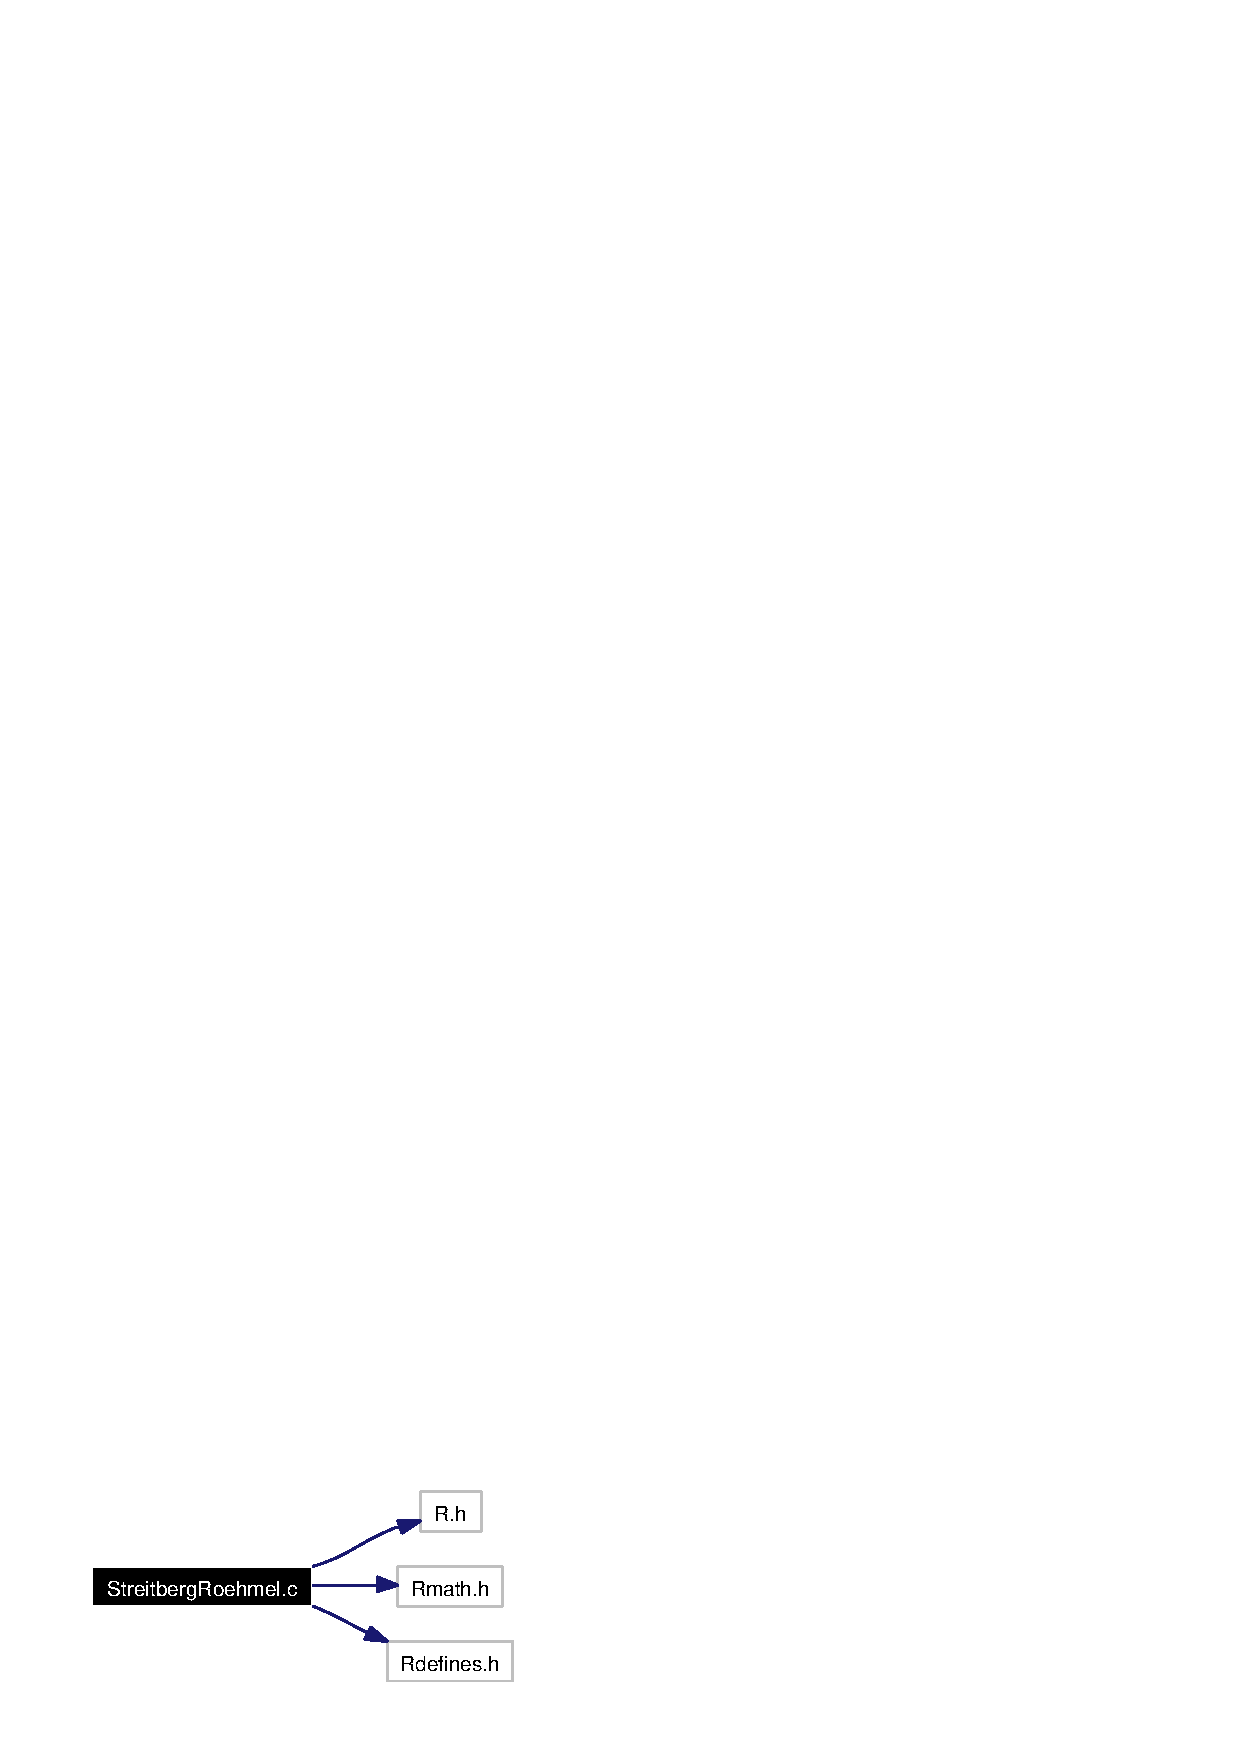
\includegraphics[width=122pt]{StreitbergRoehmel_8c__incl}
\end{center}
\end{figure}
\subsection*{Defines}
\begin{CompactItemize}
\item 
\#define \hyperlink{StreitbergRoehmel_8c_a5789a1eaa89d3dacbc12e9c27f4f622}{PERM\_\-MAX\_\-N}~1000000
\end{CompactItemize}
\subsection*{Functions}
\begin{CompactItemize}
\item 
SEXP \hyperlink{StreitbergRoehmel_8c_f9a845b0ec4e288550ee071a11d42e3f}{R\_\-cpermdist2} (SEXP score\_\-a, SEXP score\_\-b, SEXP m\_\-a, SEXP m\_\-b, SEXP ret\-Prob)
\item 
SEXP \hyperlink{StreitbergRoehmel_8c_5bccf6c77bf2cabd9930b24d7fac273a}{R\_\-cpermdist1} (SEXP scores)
\end{CompactItemize}


\subsection{Detailed Description}
Exact Distribution of Two-Sample Permutation Tests Streitberg \& Roehmel Algorithm

\begin{Desc}
\item[Author:]\begin{Desc}
\item[Author]hothorn \end{Desc}
\end{Desc}
\begin{Desc}
\item[Date:]\begin{Desc}
\item[Date]2005-07-28 17:04:29 +0200 (Thu, 28 Jul 2005) \end{Desc}
\end{Desc}


Definition in file \hyperlink{StreitbergRoehmel_8c-source}{Streitberg\-Roehmel.c}.

\subsection{Define Documentation}
\hypertarget{StreitbergRoehmel_8c_a5789a1eaa89d3dacbc12e9c27f4f622}{
\index{StreitbergRoehmel.c@{Streitberg\-Roehmel.c}!PERM_MAX_N@{PERM\_\-MAX\_\-N}}
\index{PERM_MAX_N@{PERM\_\-MAX\_\-N}!StreitbergRoehmel.c@{Streitberg\-Roehmel.c}}
\subsubsection[PERM\_\-MAX\_\-N]{\setlength{\rightskip}{0pt plus 5cm}\#define PERM\_\-MAX\_\-N~1000000}}
\label{StreitbergRoehmel_8c_a5789a1eaa89d3dacbc12e9c27f4f622}




Definition at line 19 of file Streitberg\-Roehmel.c.

Referenced by R\_\-cpermdist1(), and R\_\-cpermdist2().

\subsection{Function Documentation}
\hypertarget{StreitbergRoehmel_8c_5bccf6c77bf2cabd9930b24d7fac273a}{
\index{StreitbergRoehmel.c@{Streitberg\-Roehmel.c}!R_cpermdist1@{R\_\-cpermdist1}}
\index{R_cpermdist1@{R\_\-cpermdist1}!StreitbergRoehmel.c@{Streitberg\-Roehmel.c}}
\subsubsection[R\_\-cpermdist1]{\setlength{\rightskip}{0pt plus 5cm}SEXP R\_\-cpermdist1 (SEXP {\em scores})}}
\label{StreitbergRoehmel_8c_5bccf6c77bf2cabd9930b24d7fac273a}


The density of the permutation distribution for the one sample problem.

REFERENCES

Bernd Streitberg \& Joachim R$\backslash$\char`\"{}ohmel (1986), Exact distributions for permutations and rank tests: An introduction to some recently published algorithms. Statistical Software Newsletter 12(1), 10-17.

Bernd Streitberg \& Joachim R$\backslash$\char`\"{}ohmel (1987), Exakte Verteilungen f$\backslash$\char`\"{}ur Rang- und Randomisierungstests im allgemeinen \$c\$-Stichprobenfall. EDV in Medizin und Biologie 18(1), 12-19 (in german).

\begin{Desc}
\item[Parameters:]
\begin{description}
\item[{\em scores}]score vector (such as rank(abs(y)) for wilcoxsign\_\-test) \end{description}
\end{Desc}


Definition at line 204 of file Streitberg\-Roehmel.c.

References PERM\_\-MAX\_\-N.\hypertarget{StreitbergRoehmel_8c_f9a845b0ec4e288550ee071a11d42e3f}{
\index{StreitbergRoehmel.c@{Streitberg\-Roehmel.c}!R_cpermdist2@{R\_\-cpermdist2}}
\index{R_cpermdist2@{R\_\-cpermdist2}!StreitbergRoehmel.c@{Streitberg\-Roehmel.c}}
\subsubsection[R\_\-cpermdist2]{\setlength{\rightskip}{0pt plus 5cm}SEXP R\_\-cpermdist2 (SEXP {\em score\_\-a}, SEXP {\em score\_\-b}, SEXP {\em m\_\-a}, SEXP {\em m\_\-b}, SEXP {\em ret\-Prob})}}
\label{StreitbergRoehmel_8c_f9a845b0ec4e288550ee071a11d42e3f}


The density of the permutation distribution for the independent two sample problem.

REFERENCES

Bernd Streitberg \& Joachim R$\backslash$\char`\"{}ohmel (1986), Exact distributions for permutations and rank tests: An introduction to some recently published algorithms. Statistical Software Newsletter 12(1), 10-17.

Bernd Streitberg \& Joachim R$\backslash$\char`\"{}ohmel (1987), Exakte Verteilungen f$\backslash$\char`\"{}ur Rang- und Randomisierungstests im allgemeinen \$c\$-Stichprobenfall. EDV in Medizin und Biologie 18(1), 12-19 (in german).

\begin{Desc}
\item[Parameters:]
\begin{description}
\item[{\em score\_\-a}]score vector (typically c(1,1,...,1)) \item[{\em score\_\-b}]score vector (typically ranks) \item[{\em m\_\-a}]integer indicating the sum of m\_\-a elements of score\_\-a \item[{\em m\_\-b}]integer indicating the sum of m\_\-b elements of score\_\-b \item[{\em ret\-Prob}]logical indicating whether the density (TRUE) or the matrix of all permutations should be returned \end{description}
\end{Desc}


Definition at line 46 of file Streitberg\-Roehmel.c.

References PERM\_\-MAX\_\-N.